\chapter{Fabrication Process of CMOS}

\section{Silicon Processing}

\subsection{Why Do We Use Silicon}
We prefer Si for fabricating MOSFETs. Si is an ideal bulk semiconductor as it is easily available in large quantities, it has a bandgap of 1.12 eV which is greater than that of Germanium (0.67 eV) which means it absorbs and emits radiation in the visible region. Si can be worked at higher temperatures while Ge crystals disintegrate upon heating. Si also forms a protective SiO2 layer simply on heating which is hydrophobic in nature and eases the process of fabricating MOSFETs by acting as a barrier between bulk Si and Gate contact.



\begin{figure}[htb]
\centering
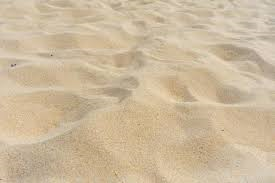
\includegraphics[scale=0.6]{./fig1} % e.g. insert ./image for image.png in the working directory, adjust scale as necessary
\caption{Silicon is widely available in nature in the form of sand}
\label{3.1} % insert suitable label, this is used to refer to a fig from within the text as shown above
\end{figure}

\subsection{Process of obtaining Silicon}
First step is simple, we reduce silica sand obtained from nature with coke to obtain Metallurgical Grade Silicon (MGS) of 98% purity.
We then treat MGS with hydrochloric acid to obtain Trichlorosilane. Impurities in MGS are converted to FeCl3, BCl3, PCl3/ PCl5 which can be removed by distillation. 
Trichlorosilane on further hydrogenation produces Si. This gives us highly pure silicon called Electronic Grade Silicon (EGS).

\subsection{Silicon Wafering }
We use the EGS obtained to produce wafers. We melt EGS in a crucible and inject a Si seed of a known orientation and rotate it and pull out the silicon melt at a slow rate. It is necessary for it to be a slow rate so that the silicon melt crystallises into the crystal of the same orientation as the seed without deformities and defects. 



\begin{figure}[htb]
\centering
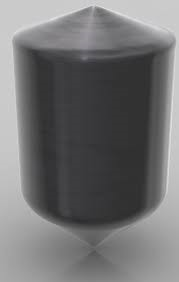
\includegraphics[scale=0.4]{./fig2} % e.g. insert ./image for image.png in the working directory, adjust scale as necessary
\caption{A Silicon ingot}
\label{3.2} % insert suitable label, this is used to refer to a fig from within the text as shown above
\end{figure}

\noindent Once the silicon ingot is obtained, we confirm crystal orientation using X-ray diffraction. We then grind a flat or notch on the ingot for the desired crystal orientation and saw it into wafers. We remove surface taper by lapping. As Si is brittle it is essential for there to be no cracks as they propagate through the entire surface. Therefore, we smoothen the edges using edge smoothening. After this we use laser scribing to ID the wafer and then etch it to remove damages caused by lapping and then polish it. Polishing allows us to thin the wafers further and remove contaminants on the surface.



\begin{figure}[htb]
\centering
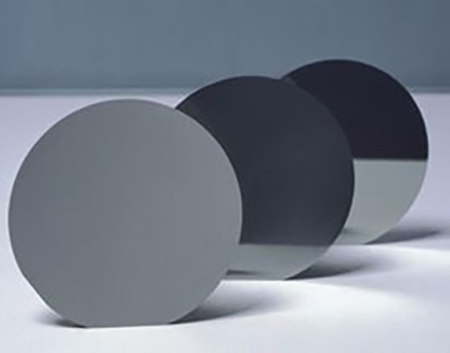
\includegraphics[scale=0.3]{./fig3} % e.g. insert ./image for image.png in the working directory, adjust scale as necessary
\caption{A Silicon wafer}
\label{fig:label} % insert suitable label, this is used to refer to a fig from within the text as shown above
\end{figure}

\pagebreak


\section{CMOS Fabrication}
In CMOS fabrication we start with a Si layer that is either p-type or n-type. Let us consider a p-type substrate in our case. 

\begin{figure}[htb]
\centering
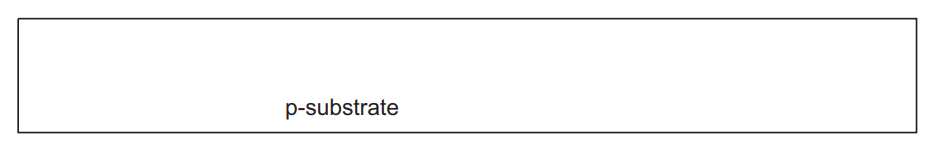
\includegraphics[scale=0.3]{./fig4} % e.g. insert ./image for image.png in the working directory, adjust scale as necessary
\caption{bare wafer}
\label{3.4} % insert suitable label, this is used to refer to a fig from within the text as shown above
\end{figure}

 
\noindent It is heated in a furnace to form a protective layer of SiO2. 

\begin{figure}[htb]
\centering
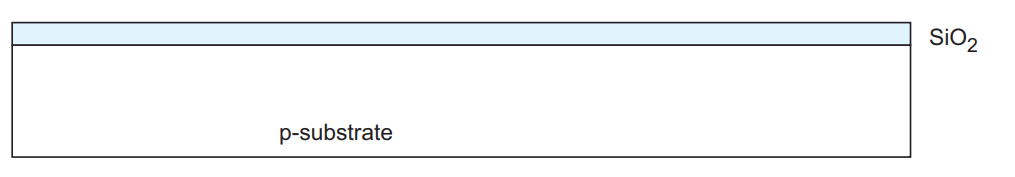
\includegraphics[scale=0.3]{./fig5} % e.g. insert ./image for image.png in the working directory, adjust scale as necessary
\caption{Oxide coating}
\label{3.5} % insert suitable label, this is used to refer to a fig from within the text as shown above
\end{figure}
 
\noindent We then add a photoresist over this layer. 

\begin{figure}[htb]
\centering
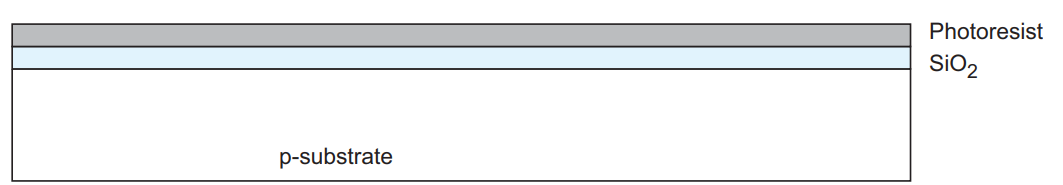
\includegraphics[scale=0.3]{./fig6} % e.g. insert ./image for image.png in the working directory, adjust scale as necessary
\caption{Photoresist coating}
\label{3.6} % insert suitable label, this is used to refer to a fig from within the text as shown above
\end{figure}
 
\noindent Say we wish to create an n-well in the bulk Si for fabricating the pMOS. We create the mask for n-well and expose the photoresist through it making it soluble in that masked area. 
\begin{figure}[H]
\centering
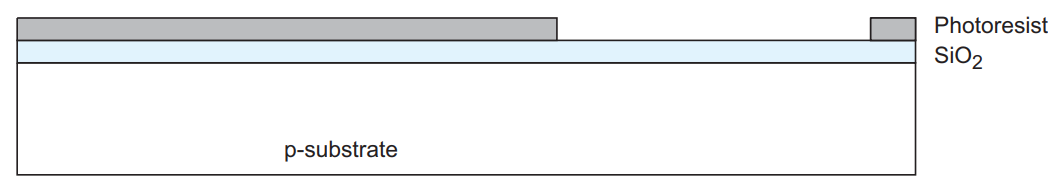
\includegraphics[scale=0.3]{./fig7} % e.g. insert ./image for image.png in the working directory, adjust scale as necessary
\caption{Masking and Etching}
\label{3.7} % insert suitable label, this is used to refer to a fig from within the text as shown above
\end{figure}
 




\noindent We etch out SiO2 layer using HF to expose the bulk Si.

\begin{figure}[H]
\centering
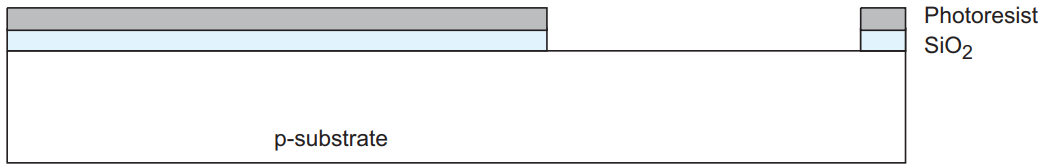
\includegraphics[scale=0.3]{./fig8} % e.g. insert ./image for image.png in the working directory, adjust scale as necessary
\caption{Oxide Etching}
\label{3.8} % insert suitable label, this is used to refer to a fig from within the text as shown above
\end{figure}
 

\noindent The remaining photoresist is removed using piranha etch.

\begin{figure}[H]
\centering
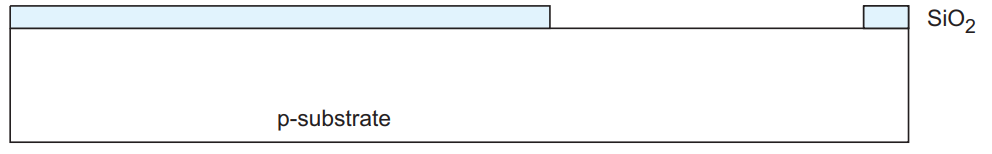
\includegraphics[scale=0.3]{./fig9} % e.g. insert ./image for image.png in the working directory, adjust scale as necessary
\caption{PR washing}
\label{3.9} % insert suitable label, this is used to refer to a fig from within the text as shown above
\end{figure}
 
\noindent We then add the n-type dopants by diffusion or ion implantation. Ion implantation provides us with the benefits of anisotropy and no lateral diffusion of dopants and better control over dopant depth.

\begin{figure}[htb]
\centering
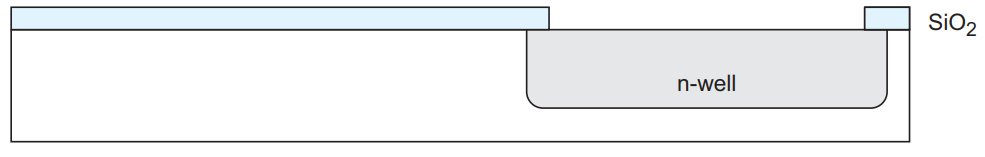
\includegraphics[scale=0.3]{./fig10} % e.g. insert ./image for image.png in the working directory, adjust scale as necessary
\caption{Ion Implantation}
\label{3.10} % insert suitable label, this is used to refer to a fig from within the text as shown above
\end{figure}
 
\noindent Excess SiO2 is removed using HF.
\begin{figure}[htb]
\centering
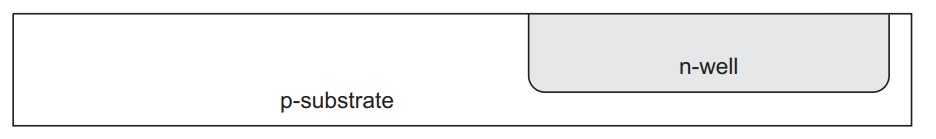
\includegraphics[scale=0.3]{./fig11} % e.g. insert ./image for image.png in the working directory, adjust scale as necessary
\caption{Etching}
\label{3.11} % insert suitable label, this is used to refer to a fig from within the text as shown above
\end{figure}
 
\noindent This gives us a Si wafer with an n-well and now we are left with generation of metal contacts and source and drain diffusion.
We once again heat the Si wafer to form SiO2. Heavily doped polysilicon is coated over SiO2 by Chemical Vapour Deposition. The wafer is heated in the presence of SiH4 to obtain wafer coated with polysilicon. 
\begin{figure}[H]
\centering
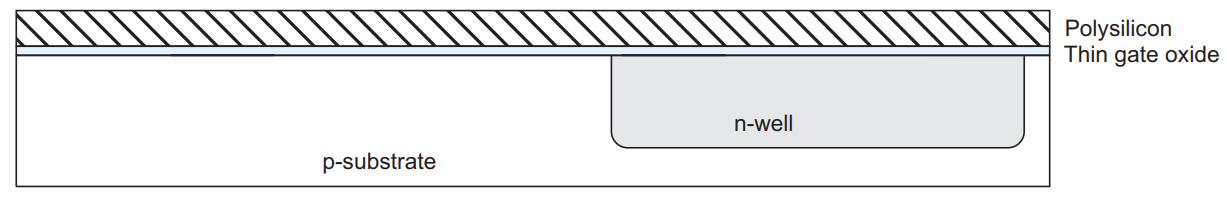
\includegraphics[scale=0.3]{./fig12} % e.g. insert ./image for image.png in the working directory, adjust scale as necessary
\caption{Polycrystalline silicon growth}
\label{3.12} % insert suitable label, this is used to refer to a fig from within the text as shown above
\end{figure}




\noindent\linebreak We pattern the area where gate contacts are to be present by using photoresist and a polysilicon mask and etch out the polysilicon and SiO2 layer from elsewhere. Leaving the gate contacts atop the oxide layer.
\begin{figure}[H]
\centering
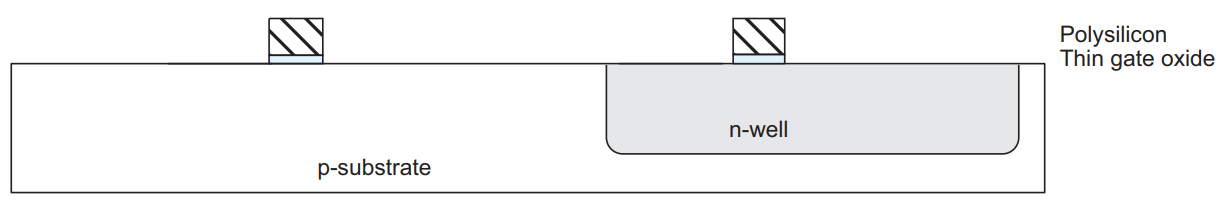
\includegraphics[scale=0.3]{./fig13} % e.g. insert ./image for image.png in the working directory, adjust scale as necessary
\caption{Gate Formation}
\label{3.13} % insert suitable label, this is used to refer to a fig from within the text as shown above
\end{figure}
 
\noindent We reheat the wafer to obtain a layer of SiO2 again and add masks in the regions where we require heavily doped n-regions for our nMOS and add dopants using the same previous method of exposure to light and etching.
\begin{figure}[H]
\centering
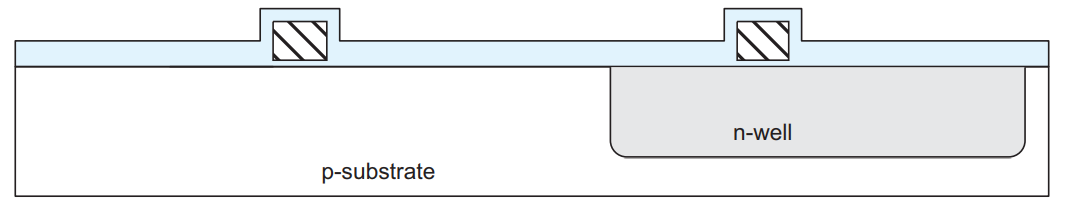
\includegraphics[scale=0.3]{./fig14} % e.g. insert ./image for image.png in the working directory, adjust scale as necessary
\caption{Oxide Growth }
\label{3.14} % insert suitable label, this is used to refer to a fig from within the text as shown above
\end{figure} 
 
\noindent We add masks to expose the region where n-type dopants are needed for the nMOS and etch out the oxide.
\begin{figure}[H]
\centering
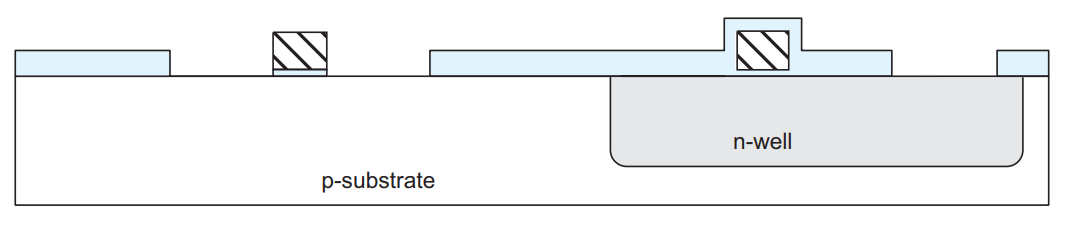
\includegraphics[scale=0.3]{./fig15} % e.g. insert ./image for image.png in the working directory, adjust scale as necessary
\caption{Source-Drain Masking and Etching}
\label{3.15} % insert suitable label, this is used to refer to a fig from within the text as shown above
\end{figure}
 
\noindent We add the n-type dopants by ion implantation. Traditionally, the dopants were diffused and therefore these regions are referred to as n-diffusion regions.
\begin{figure}[H]
\centering
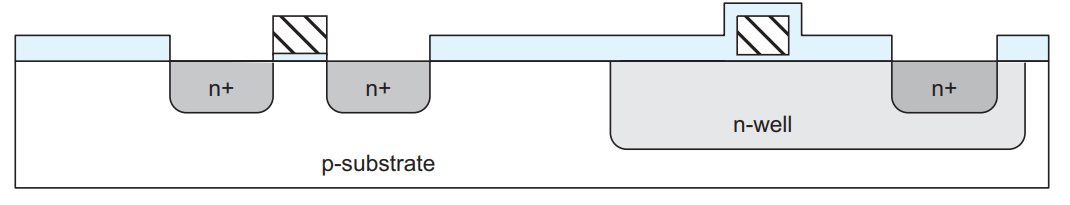
\includegraphics[scale=0.3]{./fig16} % e.g. insert ./image for image.png in the working directory, adjust scale as necessary
\caption{Dopant Implantation}
\label{3.16} % insert suitable label, this is used to refer to a fig from within the text as shown above
\end{figure}
 



\noindent We then strip off the protective oxide layer.
\begin{figure}[H]
\centering
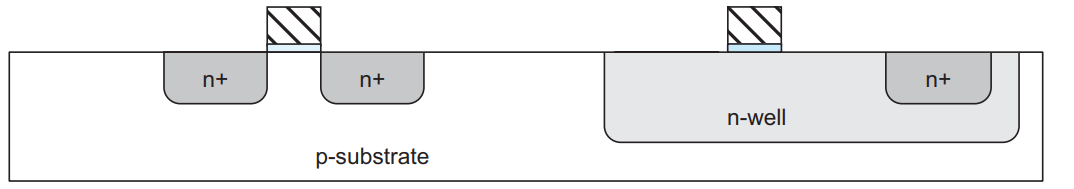
\includegraphics[scale=0.3]{./fig17} % e.g. insert ./image for image.png in the working directory, adjust scale as necessary
\caption{Oxide Etching}
\label{3.17} % insert suitable label, this is used to refer to a fig from within the text as shown above
\end{figure}
 
\noindent Similarly, we heavily dope the n-well with p type dopants to form the pMOS.
\begin{figure}[H]
\centering
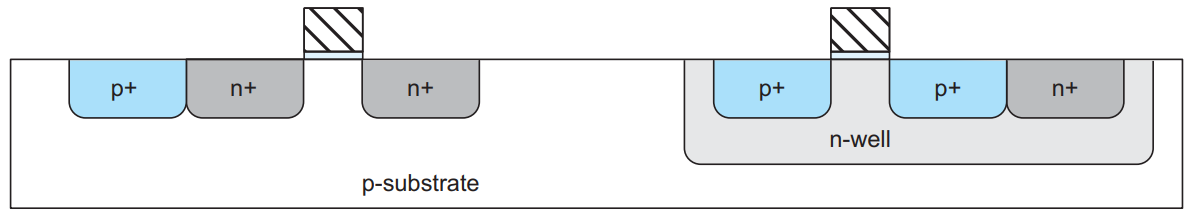
\includegraphics[scale=0.3]{./fig18} % e.g. insert ./image for image.png in the working directory, adjust scale as necessary
\caption{Fabricated CMOS}
\label{3.18} % insert suitable label, this is used to refer to a fig from within the text as shown above
\end{figure}
 
\noindent We then add masks for the metal to expose the region where metal contacts are needed.
\begin{figure}[H]
\centering
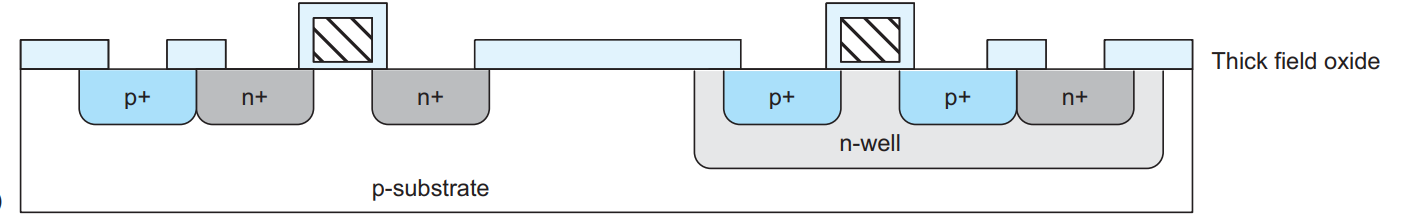
\includegraphics[scale=0.3]{./fig19} % e.g. insert ./image for image.png in the working directory, adjust scale as necessary
\caption{Fabricated CMOS}
\label{3.19} % insert suitable label, this is used to refer to a fig from within the text as shown above
\end{figure}
 
\noindent We sputter the metal over the entire wafer by blasting aluminium into vapour that evenly coats over the wafer. We use an alloy of Al and Cu. We use Cu so that Al doesn’t undergo tapering due to current flow which is a common failure mode of MOSFET called Electromigration. We remove the remaining metal from all areas by plasma etching leaving metal only where the contacts are required.
\begin{figure}[H]
\centering
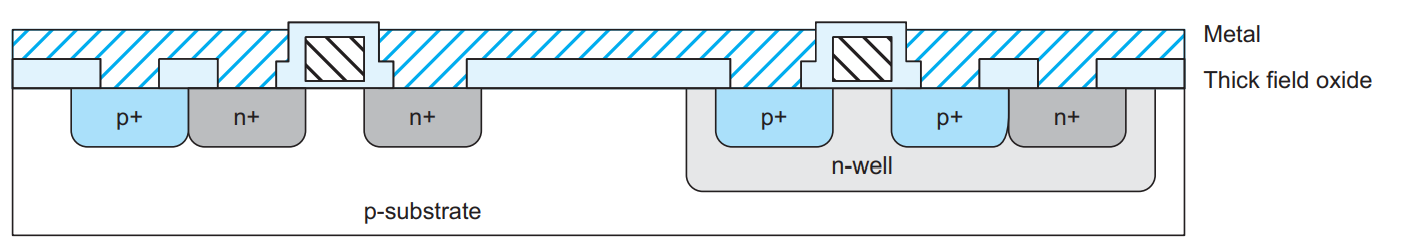
\includegraphics[scale=0.3]{./fig20} % e.g. insert ./image for image.png in the working directory, adjust scale as necessary
\caption{Fabricated CMOS with metal contacts}
\label{3.20} % insert suitable label, this is used to refer to a fig from within the text as shown above
\end{figure}







